\documentclass[aspectratio=169,xcolor=dvipsnames]{beamer}
\usetheme{SimplePlus}
\usepackage{xcolor}
\usepackage{tikz}
\usepackage{circuitikz}
\usepackage{listings}
\usepackage{amsmath}
\usepackage{amssymb}
\usepackage{tabularx}
\usepackage{booktabs}
\usepackage{multicol}
\usepackage{animate}
\usepackage{hyperref}
\usepackage{graphicx} % Allows including images
\usepackage{booktabs} % Allows the use of \toprule, \midrule and \bottomrule in tables
\usepackage[utf8]{inputenc}
\usepackage{listings}
\usepackage{xcolor}


% Theme and colors
\usecolortheme{default}
\definecolor{riscvblue}{RGB}{0.5,0.5,0.5}
\definecolor{riscvgreen}{RGB}{16,124,16}
\definecolor{riscvred}{RGB}{196,48,43}

\setbeamercolor{structure}{fg=riscvblue}
\setbeamercolor{title}{fg=riscvblue}
\setbeamercolor{frametitle}{fg=riscvblue}

% Code listing style
\lstset{
    language=Verilog,
    basicstyle=\ttfamily\small,
    keywordstyle=\color{riscvblue}\bfseries,
    commentstyle=\color{riscvgreen},
    stringstyle=\color{riscvred},
    numberstyle=\tiny\color{gray},
    numbers=left,
    stepnumber=1,
    numbersep=5pt,
    backgroundcolor=\color{gray!10},
    showspaces=false,
    showstringspaces=false,
    showtabs=false,
    frame=single,
    rulecolor=\color{black},
    tabsize=2,
    captionpos=b,
    breaklines=true,
    breakatwhitespace=false,
    title=\lstname,
    escapeinside={\%*}{*)}
}

\lstdefinelanguage{RISC-V}{
  morekeywords={addi, add, sub, lw, sw, beq, bne, jal, jalr, li, la, mv, ret, call, lui, ori, andi, slli, srai},
  sensitive=true,
  morecomment=[l]{\#},
  morestring=[b]"
}

% Title page
\title{Build your own RISC-V Processor in a Day}
\subtitle{From ISA to RTL Implementation}
\author{Maktab e Digital Systems (MEDS)}
\institute{UET Lahore}
\date{\today}

\begin{document}

\frame{\titlepage}

% Table of contents
\begin{frame}
\frametitle{Workshop Agenda}
\tableofcontents
\end{frame}

\section{Session 1: Introduction to RISC-V}

\begin{frame}
\frametitle{What is RISC-V?}
\begin{itemize}
    \item \textbf{RISC-V} = Reduced Instruction Set Computer
    \item Open-source instruction set architecture (ISA)
    \item Developed at UC Berkeley
    \item Pronounced "risk-five"
    \item Key advantages:
    \begin{itemize}
        \item Open and free
        \item Modular design
        \item Suitable for all computing domains
        \item Growing ecosystem
    \end{itemize}
\end{itemize}
\end{frame}

\begin{frame}
\frametitle{RISC-V ISA Modularity}
\begin{center}
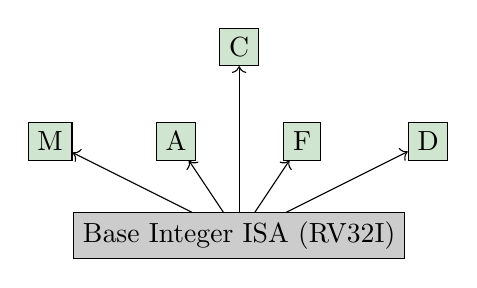
\begin{tikzpicture}[scale=0.8]
    \node[draw, rectangle, fill=riscvblue!20] (base) at (0,0) {Base Integer ISA (RV32I)};
    \node[draw, rectangle, fill=riscvgreen!20] (m) at (-3,1.5) {M};
    \node[draw, rectangle, fill=riscvgreen!20] (a) at (-1,1.5) {A};
    \node[draw, rectangle, fill=riscvgreen!20] (f) at (1,1.5) {F};
    \node[draw, rectangle, fill=riscvgreen!20] (d) at (3,1.5) {D};
    \node[draw, rectangle, fill=riscvgreen!20] (c) at (0,3) {C};
    
    \draw[->] (base) -- (m);
    \draw[->] (base) -- (a);
    \draw[->] (base) -- (f);
    \draw[->] (base) -- (d);
    \draw[->] (base) -- (c);
\end{tikzpicture}
\end{center}
\textbf{Today's Focus:} RV32I Base Integer ISA
\end{frame}

\begin{frame}
\frametitle{RISC-V Register File}
\begin{multicols}{2}
\begin{center}
\begin{tabular}{|c|c|c|}
\hline
\textbf{Register} & \textbf{ABI Name} & \textbf{Description} \\
\hline
x0 & zero & Always zero \\
x1 & ra & Return address \\
x2 & sp & Stack pointer \\
x3 & gp & Global pointer \\
x4 & tp & Thread pointer \\
x5-x7 & t0-t2 & Temporary \\
x8 & s0/fp & Saved/Frame pointer \\
x9 & s1 & Saved register \\
x10-x11 & a0-a1 & Arguments/return \\
x12-x17 & a2-a7 & Arguments \\
x18-x27 & s2-s11 & Saved registers \\
x28-x31 & t3-t6 & Temporary \\
\hline
\end{tabular}
\end{center}
\columnbreak
\begin{itemize}
    \item 32 registers in RV32I
    \item Each register is 32 bits wide
    \item x0 is hardwired to zero
    \item ABI names for software compatibility
    \item Today we'll use x0-x31 notation
\end{itemize}
\end{multicols}
\end{frame}

\begin{frame}
\frametitle{RISC-V Instruction Formats}
\begin{center}
\begin{figure}
    \centering
    \includegraphics[width=1.0\linewidth]{image.png}
    \caption{RISC-V Instruction Format}
    \label{fig:enter-label}
\end{figure}
\end{center}
\end{frame}

\begin{frame}
\frametitle{Our Subset of RV32I Instructions}
\begin{multicols}{2}
\textbf{Arithmetic \& Logic (R-type):}
\begin{itemize}
    \item \texttt{add rd, rs1, rs2}
    \item \texttt{sub rd, rs1, rs2}
    \item \texttt{and rd, rs1, rs2}
    \item \texttt{or rd, rs1, rs2}
    \item \texttt{xor rd, rs1, rs2}
    \item \texttt{slt rd, rs1, rs2}
\end{itemize}

\textbf{Immediate (I-type):}
\begin{itemize}
    \item \texttt{addi rd, rs1, imm}
    \item \texttt{andi rd, rs1, imm}
    \item \texttt{ori rd, rs1, imm}
    \item \texttt{xori rd, rs1, imm}
    \item \texttt{slti rd, rs1, imm}
\end{itemize}

\columnbreak

\textbf{Memory (I/S-type):}
\begin{itemize}
    \item \texttt{lw rd, offset(rs1)}
    \item \texttt{sw rs2, offset(rs1)}
\end{itemize}

\textbf{Branch (B-type):}
\begin{itemize}
    \item \texttt{beq rs1, rs2, offset}
    \item \texttt{bne rs1, rs2, offset}
    \item \texttt{blt rs1, rs2, offset}
    \item \texttt{bge rs1, rs2, offset}
\end{itemize}

\textbf{Jump (J-type):}
\begin{itemize}
    \item \texttt{jal rd, offset}
\end{itemize}
\end{multicols}
\end{frame}

\begin{frame}
\frametitle{Instruction Encoding Examples}
\textbf{Example 1:} \texttt{add x1, x2, x3}
\begin{center}
\begin{tabular}{|c|c|c|c|c|c|}
\hline
funct7 & rs2 & rs1 & funct3 & rd & opcode \\
\hline
0000000 & 00011 & 00010 & 000 & 00001 & 0110011 \\
\hline
\end{tabular}
\end{center}
Machine code: \texttt{0x003100B3}

\vspace{1em}
\textbf{Example 2:} \texttt{addi x1, x2, 100}
\begin{center}
\begin{tabular}{|c|c|c|c|c|}
\hline
imm[11:0] & rs1 & funct3 & rd & opcode \\
\hline
000001100100 & 00010 & 000 & 00001 & 0010011 \\
\hline
\end{tabular}
\end{center}
Machine code: \texttt{0x06410093}
\end{frame}

\section{Session 2: Assembly Programming}

\begin{frame}[fragile]
\frametitle{C to Assembly: Basic Operations}
\begin{multicols}{2}
\textbf{C Code:}
\begin{lstlisting}[language=C]
int a = 5;
int b = 10;
int c = a + b;
\end{lstlisting}

\columnbreak

\textbf{RISC-V Assembly:}

\begin{lstlisting}[language=RISC-V]
addi x1, x0, 5    # a = 5
addi x2, x0, 10   # b = 10
add  x3, x1, x2   # c = a + b
\end{lstlisting}

\end{multicols}

\textbf{Key Points:}
\begin{itemize}
    \item Variables map to registers
    \item Constants use immediate instructions
    \item \texttt{x0} is always zero (useful for loading immediates)
\end{itemize}
\end{frame}

\begin{frame}[fragile]
\frametitle{C to Assembly: Conditional Statements}
\begin{multicols}{2}
\textbf{C Code:}
\begin{lstlisting}[language=C]
if (a == b) {
    c = a + b;
} else {
    c = a - b;
}
\end{lstlisting}

\columnbreak

\textbf{RISC-V Assembly:}
\begin{lstlisting}[language=RISC-V]
beq x1, x2, equal
sub x3, x1, x2    # else case
jal x0, end       # skip equal
equal:
add x3, x1, x2    # if case
end:
\end{lstlisting}
\end{multicols}

\vspace{1em}
\textbf{Key Points:}
\begin{itemize}
    \item Conditional branches test conditions
    \item Unconditional jumps for control flow
    \item Labels mark target addresses
\end{itemize}
\end{frame}

\begin{frame}[fragile]
\frametitle{C to Assembly: Loops}
\begin{multicols}{2}
\textbf{C Code:}
\begin{lstlisting}[language=C]
int sum = 0;
for (int i = 0; i < 10; i++) {
    sum = sum + i;
}
\end{lstlisting}

\columnbreak

\textbf{RISC-V Assembly:}
\begin{lstlisting}[language={}]
addi x1, x0, 0    # sum = 0
addi x2, x0, 0    # i = 0
addi x3, x0, 10   # limit = 10
loop:
bge  x2, x3, end  # if i >= 10, exit
add  x1, x1, x2   # sum += i
addi x2, x2, 1    # i++
jal  x0, loop     # repeat
end:
\end{lstlisting}
\end{multicols}
\end{frame}

\begin{frame}[fragile]
\frametitle{Memory Operations}
\begin{multicols}{2}
\textbf{C Code:}
\begin{lstlisting}[language=C]
int arr[5] = {1, 2, 3, 4, 5};
int x = arr[2];
arr[3] = x + 1;
\end{lstlisting}

\columnbreak

\textbf{RISC-V Assembly:}
\begin{lstlisting}[language={}]
# Assume arr base in x10
lw  x1, 8(x10)    # x = arr[2]
addi x2, x1, 1    # x + 1
sw  x2, 12(x10)   # arr[3] = x + 1
\end{lstlisting}
\end{multicols}

\vspace{1em}
\textbf{Key Points:}
\begin{itemize}
    \item Array indexing uses byte addressing
    \item Each integer = 4 bytes
    \item \texttt{arr[i]} → \texttt{offset = i * 4}
\end{itemize}
\end{frame}

\begin{frame}[fragile]
\frametitle{Assembly to Machine Code}
\textbf{Step 1: Resolve Labels}
\begin{lstlisting}[language={}]
0x0000: addi x1, x0, 0    # sum = 0
0x0004: addi x2, x0, 0    # i = 0
0x0008: addi x3, x0, 10   # limit = 10
0x000C: bge  x2, x3, 0x001C  # loop: if i >= 10, exit
0x0010: add  x1, x1, x2   # sum += i
0x0014: addi x2, x2, 1    # i++
0x0018: jal  x0, 0x000C   # jump to loop
0x001C: # end:
\end{lstlisting}

\textbf{Step 2: Encode Instructions}
\begin{itemize}
    \item \texttt{addi x1, x0, 0} → \texttt{0x00000093}
    \item \texttt{bge x2, x3, 0x14} → \texttt{0x0031D863}
    \item \texttt{jal x0, 0x000C} → \texttt{0xFF5FF06F}
\end{itemize}
\end{frame}

\begin{frame}[fragile]
\frametitle{Creating Instruction Memory}
\textbf{Memory Initialization File (mem.hex):}
\begin{lstlisting}[language={}]
00000093  // addi x1, x0, 0
00000113  // addi x2, x0, 0
00A00193  // addi x3, x0, 10
0031D863  // bge x2, x3, 20
002080B3  // add x1, x1, x2
00110113  // addi x2, x2, 1
FF5FF06F  // jal x0, -12
\end{lstlisting}

\end{frame}

\begin{frame}[fragile]
\frametitle{Creating Instruction Memory}

\textbf{In SystemVerilog:}
\begin{lstlisting}[language=Verilog]
module instruction_memory (
    input  logic [31:0] addr,
    output logic [31:0] instruction
);
    logic [31:0] mem [0:1023];
    
    initial begin
        $readmemh("mem.hex", mem);
    end
    
    assign instruction = mem[addr[31:2]];
endmodule
\end{lstlisting}
\end{frame}


\section{Session 3: Processor Architecture}

\begin{frame}
\frametitle{Single-Cycle Processor Overview}
\begin{center}
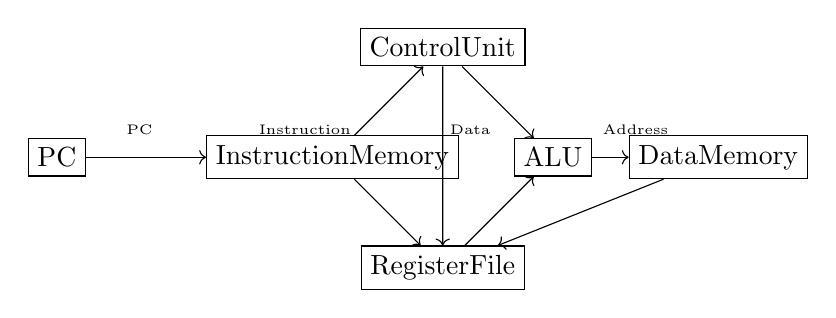
\begin{tikzpicture}[scale=0.7]
    % Program Counter
    \node[draw, rectangle] (pc) at (0,0) {PC};
    
    % Instruction Memory
    \node[draw, rectangle] (imem) at (5,0) {Instruction\\Memory};
    
    % Control Unit
    \node[draw, rectangle] (ctrl) at (7,2) {Control\\Unit};
    
    % Register File
    \node[draw, rectangle] (rf) at (7,-2) {Register\\File};
    
    % ALU
    \node[draw, rectangle] (alu) at (9,0) {ALU};
    
    % Data Memory
    \node[draw, rectangle] (dmem) at (12,0) {Data\\Memory};
    
    % Connections
    \draw[->] (pc) -- (imem);
    \draw[->] (imem) -- (ctrl);
    \draw[->] (imem) -- (rf);
    \draw[->] (ctrl) -- (rf);
    \draw[->] (ctrl) -- (alu);
    \draw[->] (rf) -- (alu);
    \draw[->] (alu) -- (dmem);
    \draw[->] (dmem) -- (rf);
    
    % Labels
    \node at (1.5,0.5) {\tiny PC};
    \node at (4.5,0.5) {\tiny Instruction};
    \node at (7.5,0.5) {\tiny Data};
    \node at (10.5,0.5) {\tiny Address};
    
\end{tikzpicture}
\end{center}

\textbf{Key Components:}
\begin{itemize}
    \item Program Counter (PC)
    \item Instruction Memory
    \item Control Unit
    \item Register File
    \item ALU
    \item Data Memory
\end{itemize}
\end{frame}

\begin{frame}
\frametitle{Instruction Fetch, Decode, Execute}
\begin{enumerate}
    \item \textbf{Fetch:} Read instruction from memory at PC address
    \item \textbf{Decode:} 
    \begin{itemize}
        \item Extract fields (opcode, rs1, rs2, rd, immediate)
        \item Generate control signals
        \item Read register file
    \end{itemize}
    \item \textbf{Execute:}
    \begin{itemize}
        \item Perform ALU operation
        \item Access data memory (if needed)
        \item Write back to register file
        \item Update PC
    \end{itemize}
\end{enumerate}

\vspace{1em}
\textbf{Single-Cycle:} All steps complete in one clock cycle
\end{frame}

\begin{frame}
\frametitle{Detailed Datapath}
\begin{center}
\begin{figure}
    \centering
    \includegraphics[width=0.5\linewidth]{datapath.png}
    \caption{RISC-V Datapath}
    \label{fig:enter-label}
\end{figure}
\end{center}
\end{frame}

\begin{frame}
\frametitle{Control Unit Design}
\begin{center}
\scriptsize
\begin{tabular}{|c|c|c|c|c|c|c|c|}
\hline
\textbf{Instruction} & \textbf{RegWrite} & \textbf{ALUSrc} & \textbf{MemRead} & \textbf{MemWrite} & \textbf{Branch} & \textbf{MemtoReg} & \textbf{ALUOp} \\
\hline
R-type & 1 & 0 & 0 & 0 & 0 & 0 & 10 \\
I-type (ALU) & 1 & 1 & 0 & 0 & 0 & 0 & 10 \\
Load & 1 & 1 & 1 & 0 & 0 & 1 & 00 \\
Store & 0 & 1 & 0 & 1 & 0 & X & 00 \\
Branch & 0 & 0 & 0 & 0 & 1 & X & 01 \\
\hline
\end{tabular}
\end{center}

\vspace{1em}
\textbf{Control Signal Functions:}
\begin{itemize}
    \item \textbf{RegWrite:} Enable register file write
    \item \textbf{ALUSrc:} Select ALU input (register vs immediate)
    \item \textbf{MemRead/MemWrite:} Enable data memory operations
    \item \textbf{Branch:} Enable branch condition check
    \item \textbf{MemtoReg:} Select register write data source
    \item \textbf{ALUOp:} ALU operation type
\end{itemize}
\end{frame}

\begin{frame}
\frametitle{ALU Control}
\begin{center}
\begin{tabular}{|c|c|c|c|}
\hline
\textbf{ALUOp} & \textbf{Funct3} & \textbf{Funct7[5]} & \textbf{ALU Control} \\
\hline
00 & XXX & X & 0010 (add) \\
01 & XXX & X & 0110 (sub) \\
10 & 000 & 0 & 0010 (add) \\
10 & 000 & 1 & 0110 (sub) \\
10 & 001 & X & 0000 (and) \\
10 & 010 & X & 0001 (or) \\
10 & 100 & X & 0100 (xor) \\
10 & 101 & X & 0111 (slt) \\
\hline
\end{tabular}
\end{center}

\end{frame}

\begin{frame}
\frametitle{ALU Control}
\textbf{ALU Operations:}
\begin{itemize}
    \item 0000: AND
    \item 0001: OR
    \item 0010: ADD
    \item 0100: XOR
    \item 0110: SUB
    \item 0111: SLT (Set Less Than)
\end{itemize}
\end{frame}

\section{Session 4: RTL Implementation}

\begin{frame}[fragile]
\frametitle{Top-Level Processor Module}
\begin{lstlisting}[language=Verilog]
module processor (
    input  logic clk,
    input  logic reset,
    output logic [31:0] pc_out,
    output logic [31:0] instruction_out
);
    
\end{lstlisting}
\end{frame}

\begin{frame}[fragile]
\frametitle{Top-Level Processor Module}
\begin{lstlisting}[language=Verilog]
    // Datapath Signals    
    logic [31:0] pc, pc_next, pc_plus_4;
    logic [31:0] instruction;
    logic [31:0] read_data1, read_data2, write_data;
    logic [31:0] alu_result, mem_read_data;
    logic [31:0] immediate;
    logic [4:0] rs1, rs2, rd;
    logic [6:0] opcode;
    logic [2:0] funct3;
    logic [6:0] funct7;
\end{lstlisting}
\end{frame}

\begin{frame}[fragile]
\frametitle{Top-Level Processor Module}
\begin{lstlisting}[language=Verilog]
    
    
    // Control signals
    logic reg_write, alu_src, mem_read, mem_write;
    logic branch, mem_to_reg, jump;
    logic [3:0] alu_control;
    logic zero_flag;
    
    // Instantiate modules here...
    
endmodule
\end{lstlisting}
\end{frame}


\begin{frame}[fragile]
\frametitle{Register File Implementation}
\begin{lstlisting}[language=Verilog]
module register_file (
    input  logic        clk,
    input  logic        reset,
    input  logic [4:0]  read_addr1,
    input  logic [4:0]  read_addr2,
    input  logic [4:0]  write_addr,
    input  logic [31:0] write_data,
    input  logic        write_enable,
    output logic [31:0] read_data1,
    output logic [31:0] read_data2
);
    
\end{lstlisting}
\end{frame}

\begin{frame}[fragile]
\frametitle{Register File Implementation}
\begin{lstlisting}[language=Verilog]
    
    logic [31:0] registers [0:31];
    
    // x0 is always zero
    assign registers[0] = 32'h0;
    
    // Read operations (combinational)
    assign read_data1 = registers[read_addr1];
    assign read_data2 = registers[read_addr2];
    
\end{lstlisting}
\end{frame}

\begin{frame}[fragile]
\frametitle{Register File Implementation}
\begin{lstlisting}[language=Verilog]
    
    
    // Write operation (sequential)
    always_ff @(posedge clk) begin
        if (reset) begin
            for (int i = 1; i < 32; i++) begin
                registers[i] <= 32'h0;
            end
        end else if (write_enable && write_addr != 0) begin
            registers[write_addr] <= write_data;
        end
    end
    
endmodule
\end{lstlisting}
\end{frame}


\begin{frame}[fragile]
\frametitle{ALU Implementation}
\begin{lstlisting}[language=Verilog]
module alu (
    input  logic [31:0] operand_a,
    input  logic [31:0] operand_b,
    input  logic [3:0]  alu_control,
    output logic [31:0] result,
    output logic        zero
);
\end{lstlisting}
\end{frame}


\begin{frame}[fragile]
\frametitle{ALU Implementation}
\begin{lstlisting}[language=Verilog]
    
    always_comb begin
        case (alu_control)
            4'b0000: result = operand_a & operand_b;      // AND
            4'b0001: result = operand_a | operand_b;      // OR
            4'b0010: result = operand_a + operand_b;      // ADD
            4'b0100: result = operand_a ^ operand_b;      // XOR
            4'b0110: result = operand_a - operand_b;      // SUB
            4'b0111: result = (operand_a < operand_b) ? 1 : 0; // SLT
            default: result = 32'h0;
        endcase
    end
    
    assign zero = (result == 32'h0);
    
endmodule
\end{lstlisting}
\end{frame}

\begin{frame}[fragile]
\frametitle{Control Unit Implementation}
\begin{lstlisting}[language=Verilog]
module control_unit (
    input  logic [6:0] opcode,
    input  logic [2:0] funct3,
    input  logic [6:0] funct7,
    output logic       reg_write,
    output logic       alu_src,
    output logic       mem_read,
    output logic       mem_write,
    output logic       branch,
    output logic       mem_to_reg,
    output logic       jump,
    output logic [3:0] alu_control
);
    
\end{lstlisting}
\end{frame}


\begin{frame}[fragile]
\frametitle{Control Unit Implementation}
\begin{lstlisting}[language=Verilog]
    
    logic [1:0] alu_op;
    
    // Main control signals
    always_comb begin
        case (opcode)
            7'b0110011: begin // R-type
                reg_write = 1; alu_src = 0; mem_read = 0;
                mem_write = 0; branch = 0; mem_to_reg = 0;
                jump = 0; alu_op = 2'b10;
            end
            // Add more cases...
            default: begin
                reg_write = 0; alu_src = 0; mem_read = 0;
                mem_write = 0; branch = 0; mem_to_reg = 0;
                jump = 0; alu_op = 2'b00;
            end
        endcase
    end
    
    // ALU control logic
    // ... (implement ALU control based on alu_op, funct3, funct7)
    
endmodule
\end{lstlisting}
\end{frame}



\begin{frame}[fragile]
\frametitle{Immediate Generation}
\begin{lstlisting}[language=Verilog]
module immediate_generator (
    input  logic [31:0] instruction,
    input  logic [6:0]  opcode,
    output logic [31:0] immediate
);
    
\end{lstlisting}
\end{frame}


\begin{frame}[fragile]
\frametitle{Immediate Generation}
\begin{lstlisting}[language=Verilog]
    
    always_comb begin
        case (opcode)
            7'b0010011: begin // I-type
                immediate = {{20{instruction[31]}}, instruction[31:20]};
            end
            7'b0100011: begin // S-type
                immediate = {{20{instruction[31]}}, 
                           instruction[31:25], instruction[11:7]};
            end
            default: immediate = 32'h0;
        endcase
    end
    
endmodule
\end{lstlisting}
\end{frame}



\section{Session 5: Verification \& Testing}

\begin{frame}[fragile]
\frametitle{Testbench Structure}
\begin{lstlisting}[language=Verilog]
module tb_processor;
    logic clk, reset;
    logic [31:0] pc_out, instruction_out;
    
    // Instantiate processor
    processor dut (
        .clk(clk),
        .reset(reset),
        .pc_out(pc_out),
        .instruction_out(instruction_out)
    );
    
\end{lstlisting}
\end{frame}

\begin{frame}[fragile]
\frametitle{Testbench Structure}
\begin{lstlisting}[language=Verilog]
    // Clock generation
    initial begin
        clk = 0;
        forever #5 clk = ~clk;
    end
    
    // Test sequence
    initial begin
        reset = 1;
        #10 reset = 0;
        
\end{lstlisting}
\end{frame}


\begin{frame}[fragile]
\frametitle{Testbench Structure}
\begin{lstlisting}[language=Verilog]
        // Run for several cycles
        repeat (20) @(posedge clk);
        
        $finish;
    end
    
    // Monitor outputs
    initial begin
        $monitor("Time=%0t PC=%h Instruction=%h", 
                 $time, pc_out, instruction_out);
    end
    
endmodule
\end{lstlisting}
\end{frame}



\begin{frame}[fragile]
\frametitle{ALU Testbench}
\begin{lstlisting}[language=Verilog]
module tb_alu;
    logic [31:0] operand_a, operand_b, result;
    logic [3:0] alu_control;
    logic zero;
    
    // Instantiate ALU
    alu dut (.*);    
    // Test vectors
    initial begin
        $display("Testing ALU...");
        
        // Test ADD
        operand_a = 32'h10; operand_b = 32'h20; alu_control = 4'b0010;
        #10 assert(result == 32'h30) else $error("ADD failed");
        
        // Test SUB ...
\end{lstlisting}
\end{frame}


\begin{frame}
\frametitle{Workshop Summary}
\textbf{What we've accomplished:}
\begin{itemize}
    \item ✓ Understood RISC-V ISA fundamentals
    \item ✓ Converted C code to assembly
    \item ✓ Generated machine code
    \item ✓ Designed single-cycle datapath
    \item ✓ Implemented control logic
    \item ✓ Coded complete processor in SystemVerilog
    \item ✓ Verified with comprehensive testbenches
\end{itemize}

\vspace{1em}
\textbf{Next steps:}
\begin{itemize}
    \item Extend instruction set support
    \item Add pipeline stages
    \item Optimize for performance
\end{itemize}
\end{frame}

\begin{frame}
\frametitle{Performance Metrics}
\textbf{Our Single-Cycle Processor:}
\begin{itemize}
    \item \textbf{Clock Period:} Limited by longest instruction path
    \item \textbf{CPI:} 1 (Cycles Per Instruction)
    \item \textbf{Instruction Set:} 20+ RV32I instructions
    \item \textbf{Memory:} Harvard architecture (separate I/D)
    \item \textbf{Area:} Approximately 5000 gates
\end{itemize}

\vspace{1em}
\textbf{Typical Performance:}
\begin{itemize}
    \item \textbf{Frequency:} 50-100 MHz on FPGA
    \item \textbf{Throughput:} 50-100 MIPS
    \item \textbf{Power:} Low (no complex features)
    \item \textbf{Use cases:} Embedded systems, IoT, education
\end{itemize}
\end{frame}

\begin{frame}
\frametitle{Common Debug Techniques}
\textbf{Simulation Debug:}
\begin{itemize}
    \item Use \texttt{\$display} and \texttt{\$monitor} statements
    \item Add assertions for critical conditions
    \item Use waveform viewers (GTKWave, ModelSim)
    \item Check control signal timing
\end{itemize}

\vspace{1em}
\textbf{Hardware Debug:}
\begin{itemize}
    \item Add debug ports to processor
    \item Use FPGA debug cores (ILA, VIO)
    \item Implement simple serial output
    \item Use LED indicators for status
\end{itemize}

\vspace{1em}
\textbf{Common Issues:}
\begin{itemize}
    \item Incorrect immediate sign extension
    \item Wrong ALU control signals
\end{itemize}
\end{frame}

\begin{frame}
\frametitle{Questions \& Discussion}
\begin{center}
\huge{Questions?}
\end{center}

\vspace{2em}
\begin{itemize}
    \item What challenges did you face?
    \item Which part was most interesting?
    \item Ideas for processor improvements?
    \item Real-world applications?
\end{itemize}

\vspace{2em}
\begin{center}
\textbf{Thank you for attending!}

\vspace{1em}
\textit{Keep building, keep learning!}
\end{center}
\end{frame}

\begin{frame}
\frametitle{References \& Resources}
\begin{itemize}
    \item \textbf{RISC-V ISA Specification:} \\
    \url{https://riscv.org/technical/specifications/}
    
    \item \textbf{"Computer Organization and Design RISC-V Edition":} \\
    Patterson \& Hennessy
    
    \item \textbf{SystemVerilog IEEE Standard:} \\
    IEEE 1800-2017
    
    \item \textbf{Online RISC-V Simulator:} \\
    \url{https://www.cs.cornell.edu/courses/cs3410/2019sp/riscv/interpreter/}
       
    \item \textbf{Workshop GitHub Repository:} \\
    \url{https://github.com/meds-uet/rv-workshop}
\end{itemize}
\end{frame}

\end{document}